% v2-acmtog-sample.tex, dated March 7 2012
% This is a sample file for ACM Transactions on Graphics
%
% Compilation using 'acmtog.cls' - version 1.2 (March 2012), Aptara Inc.
% (c) 2010 Association for Computing Machinery (ACM)
%
% Questions/Suggestions/Feedback should be addressed to => "acmtexsupport@aptaracorp.com".
% Users can also go through the FAQs available on the journal's submission webpage.
%
% Steps to compile: latex, bibtex, latex latex
%
% For tracking purposes => this is v1.2 - March 2012
\documentclass{acmtog} % V1.2
% \usepackage{caption}
% \usepackage{graphicx, subfig}
%\acmVolume{VV}
%\acmNumber{N}
%\acmYear{YYYY}
%\acmMonth{Month}
%\acmArticleNum{XXX}
%\acmdoi{10.1145/XXXXXXX.YYYYYYY}
% \fancyfoot{\empty}
\acmVolume{}
\acmNumber{}
\acmYear{}
\acmMonth{}
\acmArticleNum{}
\acmdoi{}
\usepackage{amsmath}
\usepackage[ruled]{algorithm2e}
\begin{document}

% \markboth{V. F. Pamplona et al.}{Photorealistic Models for Pupil Light Reflex and Iridal Pattern Deformation}

\title{Text Decryption by MCMC} % title

\author{Zhengyi Li {\upshape and} Haoyu Geng
\affil{Shanghai Jiao Tong University}
% \and
% GLADIMIR V. G. BARANOSKI
% \affil{University of Waterloo}
% NOTE! Affiliations placed here should be for the institution where the
%       BULK of the research was done. If the author has gone to a new
%       institution, before publication, the (above) affiliation should NOT be changed.
%       The authors 'current' address may be given in the "Author's addresses:" block (below).
%       So for example, Mr. Fogarty, the bulk of the research was done at UIUC, and he is
%       currently affiliated with NASA.
}

% \category{I.3.7}{Cryptography}
% \category{I.3.5}{Computer Graphics}{Computational Geometry and Object Modeling}[Physically based modeling]

% \terms{Experimentation, Human Factors}

% \keywords{Face animation, image-based modelling, iris animation, photorealism, physiologically-based modelling}

% \acmformat{Vitor F. Pamplona, Manuel M. Oliveira, Gladimir V. G. Baranoski,
% and Sean Fogarty. 2009. Photorealistic models for pupil light reflex and iridal pattern deformation.
% {\em ACM Trans. Graph.} 28, 4, Article 106 (September 2009), 10 pages.\\
% \doiline}


\maketitle

\begin{abstract}
    In this paper, we used a method to break the substitution cipher by combining the method of MCMC(Monte Carlo Markov Chain) and local search, with linear time complexity and the accuracy above 99\%. Besides, we proposed new methods to speed up the process of convergence by \textbf{variable exploring method}, and also reduce the search space by \textbf{double search}, and mede some efforts in memory optimization and new evaluation function.
\end{abstract}
\tableofcontents

\newpage

% \begin{bottomstuff}
% Manuel M. Oliveira acknowledges a CNPq-Brazil fellowship (305613/2007-3). Gladimir V. G. Baranoski acknowledges a
% NSERC-Canada grant (238337). Microsoft Brazil provided additional support.
% Authors' addresses: Sean Fogarty, (Current address) NASA Ames Research Center, Moffett Field, California 94035.
% \end{bottomstuff}



\section{Introduction}

The method to decode the cipher is a traditional area of research in cryptography. There are many branches depending on encoding methods, and the decoding cipher of direct character substitution is one of the most classic problem. However, the traditional methods in cryptography is computationally expensive, both in spatial and temporal aspects.  \\\\
There are several papers regarding the algorithms to automatically get a solution for substitution cipher. It includes heuristic methods to search for the best deterministic key(Peleg and Rosenfeld, 1979; Ganesan and Sherman, 1993; Jakobsen, 1995; Olson,2007), which uses word dictionaries to guide the search. It also includes methods of expectation-maximization (EM) to search for the best probabilistic key using letter n-gram models (Knight et al., 2006).\\\\
In this paper, we want to develop and implement a light-weighted algorithm to solve this problem and we will focus on deciphering a piece of text in direct substitution of characters. Based on some previous effort in this area, We combined Monte Carlo Markov chain(MCMC) and local search to break the cipher. Besides, to improve the performance of this algorithm, we also devised several methods to reduce time and space complexity. we noticed some problems in the process and find some way to increase the accuracy and speed up the process of convergence. Our methods works well on the test set with different text type and text length.
\section{Background}
% \label{sec:relatedwork}
%
There is a interesting story behind our problem. One day, a piece of text appears in the prison system in California. It seems to be that the prisoners are conveying messages via the coded message, and people wanted to decipher the text. A simple speculation for this text is that the cipher is a direct character substitution, and thus researchers want to find a simple method to break the code.
\begin{figure}[ht]
  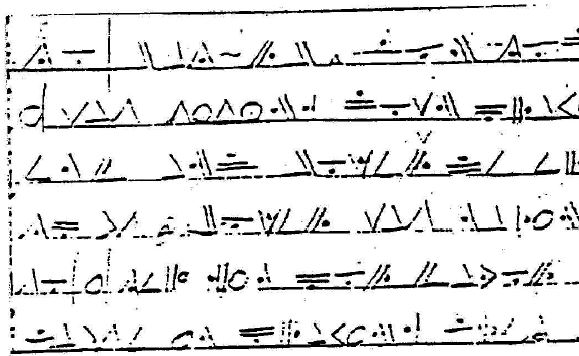
\includegraphics[width=.4\textwidth]{pic/CA.JPG} 
  \caption{cipher text found in California prison} 
  \label{CA}
\end{figure}
There are many different types of substitution cipher, and in this project, we will focus on \textbf{simple substitution cipher}, which is that the cipher operates on a single letter. Although substitution cipher is not a complicated form and relatively not difficult to break, the method of sampling method is rarely used in nowadays research, and probably this method could be expanded to other areas in cryptography.
\begin{figure}[ht]
  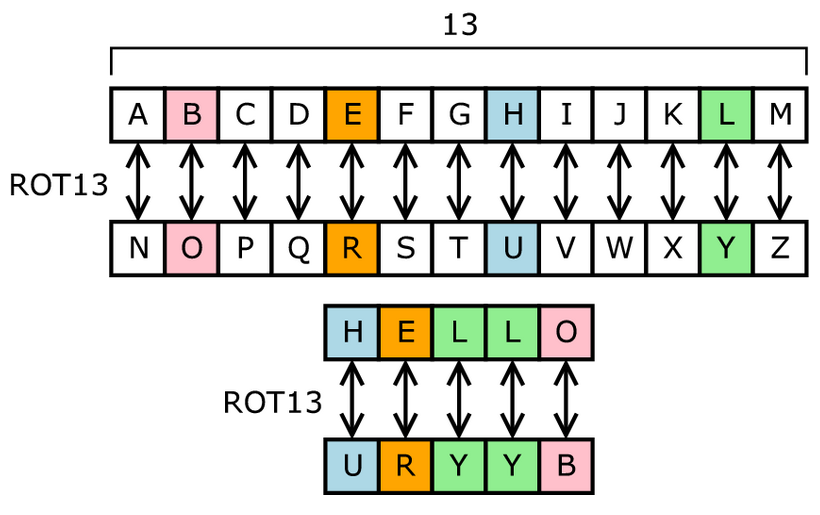
\includegraphics[width=.35\textwidth]{pic/direct.png} 
  \caption{A simple example for substitution cipher} 
  \label{direct}
\end{figure}

\section{Related Work}
% \label{sec:biologicalreview}
In Ravi and Knight et al. 2008\cite{Ravi}, it uses low-order n-gram model, and set global constraints using integer programming. In Nuhn and Schamper et al. 2013.\cite{Nuhn}, it uses beam search approach and takes high-order n-gram method. In Hauer, Hayward, Kondrak et al. 2014.\cite{Hauer}, it uses MCST(Monte Carlo search Tree) to implement an unsupervised transliteration. In the work by Stephen Connor in his paper Simulation and Solving Substitution Codes\cite{Conner}, they introduce the method using MCMC sampling and proposed random work.\\\\
In the light of the previous work, we combined MCMC sampling method with local search with low-order n-gram, and we proposed the new method to address the problems in this method and improved the performance. 
\section{Motivation}
Local search is quite famous for solving NPC problems such as TSP. Intuitively, local search will also work for decoding problem. As for MCMC, it will need some thinking to apply to decoding problem. MCMC is a set of algorithms which are used to sample complex distributions, especially those can't expressed as total probability distribution. Here, in this problem, we used Metropolis-Hastings algorithm(MH) of MCMC. You may surprised at this sample algorithm: how could it solve decoding problem? Actually, we construct this problem by endowing all the solutions a probability, and good solution own a higher probability while bad solutions own lower probability. So we can using MH to sample the solution space and finally we will derive a set of solutions closed to the real probability distribution. The correct solution appears the most times in the solution set. Next I will introduce what are MCMC and local search, and why they are suitable for this problem.
\subsection{Principle of Metropolis-Hastings algorithm}
In this part, I will introduce what is MH algorithm. However, I will not go deep into the theorem. Instead, only the parts which are correlated to this problem will be discussed.

Sometimes, we need to calculate expectation of a certain probability distribution. If the distribution is as simple as uniform distribution, the problem is quite easy. However, if the distribution is complex, even the Gauss distribution, we can't calculate a exact result since the distribution is hard to approached. Then it comes to MH. With the help of sample algorithm MH, we can sample according to the given distribution. And the obtained sample set has the same probability as the origin distribution. There are two keys:
\begin{enumerate}
    \item The sample process is a Markov chain where current state only depends on the previous state. And the new sample is proposed according to conditional probability distribution.
    \item The accept rate ${\alpha}$ is defined as this 
    \begin{center}
        ${\alpha }_{\left(x,y\right)}=min\{1,\frac{\pi \left(y\right)q\left(y,x\right)}{\pi \left(x\right)q\left(x,y\right)}\}$
    \end{center} There is also a uniform number u between (0,1). Whether to accept new sample depends on whether ${\alpha}$ greater than u. This condition is strict(which is called as detailed balance condition) to make sure the final sample set approaches real probability distribution.
\end{enumerate}
With the above two key conditions, after enough large sample iterations, we will derive a sample set which distributes like real distribution. Then we can use this sample set to fulfill the need. In this problem, the need is to find the correct solution.
\subsection{Principle of Local Search}
This method is prevalent in solving intractable problem. Local search is used by defining a state space and walk through it according to heuristic function. Although the space is extremely large, the solution can be found by heuristic functions. In this problem, we utilize local search to propose new state.
\subsection{Why we use them}
At the beginning of this part, I have mentioned a little about how we combined MH and local search to solve decoding problem. After discussing the principles of MH and local search, I am going to talk about why we use them in detail.

First, I would like to introduce how we consider the decoding problem. Any English text is a kind of Markov chain where current character is only based on the previous character. A proper two adjacent letters are more likely to emerge, which means a higher probability. And we define the entropy of a text in this way:
\begin{center}
    $entropy=-\mathrm{log}\prod _{i=0}^{N}{p}_{\left({x}_{i},{x}_{i+1}\right)}$
\end{center}
The intuition comes from the definition of entropy in information theorem. Apparently, in the probability distribution of the solutions(there exist one, but we cannot obtain it), a good solution in which the letters are in order will have a lower entropy whereas a bad solution where the letters are in chaos have a higher entropy. This means those good solution are more likely to be sampled and the bad solutions are hard to be sampled. Then after enough times iterations, the probability of an element in the sample set is close to the true probability distribution. The correct solution we need is the one appearing most times in sample set.

In traditional local search, the exploration is oblivious. So the whole process of probe is abandoned and the algorithm is end up with only a result, which is quite a pity. And you can see with the combination of MH algorithm, all the explored solution will be recorded. You can see how tricky by regarding the solution space as a probability state space and sampling from it. Despite the fact that it seems recording will take up a lot of memory space, we verified that the record is necessary and in fact, we calculate that the space complexity is not as large as we thought initially.





\label{sub:models_of_pupil_dynamics}



\section{Problem Formulation}
In our decoding problem, there are totally 56 kinds of characters, including letters, numbers, punctuation and whitespace. A encoded text is substitute each of the 56 characters with another one. After the encoding process, the text looks like a mess. Our goal is to find the substitution which has been used to encode.

At first, I will define some concepts which are useful to the problem formulation. After that, the process of the algorithm will be given.
\subsection{Definition}

\newtheorem{myDef}{Definition} 
\begin{myDef}
    Transition probability matrix P:
    \begin{center}
        $P=
        \begin{array}{lc}
	
    	\mbox{}&
    	\begin{array}{ccc}Alph_{1}&Alph_{2}&\cdots \end{array}\\
    	\begin{array}{c}Alph_{1}\\Alph_{2}\\ \vdots\end{array}&
    	\left[\begin{array}{ccc}
    		p_{11}  &  p_{12}  & \cdots\\
    		p_{21}  &  p_{22}  & \cdots\\
    		\vdots   & \vdots & \ddots  \\
    
    	\end{array}\right]
        \end{array}$
    \end{center}
    This matrix is obtained by traversing the sample text, $p_{ij}$ represents the probability of character i followed by character j after applying $\sigma$ to encoding text.
\end{myDef}

\begin{myDef}
    Transition matrix ${M}_{\sigma }$ of a permutation ${\sigma }$:
    \begin{center}
        $M_{\sigma}=
        \begin{array}{lc}
    	\mbox{}&
    	\begin{array}{ccc}Alph_{1}&Alph_{2}&\cdots \end{array}\\
    	\begin{array}{c}Alph_{1}\\Alph_{2}\\ \vdots\end{array}&
    	\left[\begin{array}{ccc}
    		m_{11}  &  m_{12}  & \cdots\\
    		m_{21}  &  m_{22}  & \cdots\\
    		\vdots   & \vdots & \ddots  \\
    
    	\end{array}\right]
        \end{array}$
    \end{center}
    Where $m_{ij}$ represents the number of character i followed by character j after applying $\sigma$ to encoding text. 
\end{myDef}

\begin{myDef}
    Permutation: A kind of substitution which represents how each of the 83 characters are replaced by another one. And if I say applying certain permutation to the encoded text, it means we change the characters according to the permutation.
\end{myDef}
\begin{myDef}
    Entropy of permutation $\varphi$: This represents the quality of a permutation after which has been applied to a text, the value is in this form:
    \begin{center}
        ${E}_{\varphi }=-\mathrm{log}\prod _{i=1}^{83}\prod _{j=1}^{83}m_{ij}p_{ij}$
    \end{center}
    the value 83 means there are 83 characters.
\end{myDef}

\begin{myDef}
    Accept rate $\alpha$: $\alpha$ is defined in this form:
    \begin{center}
        ${\alpha }_{\left(x,y\right)}=min\{1,\frac{{E}_{\varphi }}{{E}_{\sigma }}\}$
    \end{center}
    From permutation ${\varphi }$, after proposing a new state ${\sigma }$, we will use $\alpha$ to decide whether to accept it. To achieve this goal, we also need a random number from 0 to 1. If ${\alpha }_{\left(x,y\right)}$ greater than u, then accept new state ${\sigma }$. Otherwise, new state will be rejected.
\end{myDef}

\subsection{Process}
First think up a permutation randomly.
\begin{enumerate}
    \item calculate the transition matrix  under the random permutation 
    \item propose a new permutation by transposing two characters at random
    \item calculate the transition matrix of the permutation arising from the above
    transposition
    \item calculate the acceptance probability
    \item if the move is accepted, set the current transition matrix to be that found in step 3 and record this state
    \item return to step 2 until the chain converges or the maximum number of
    iterations is reached
    \item take the permutation that appears the most in the recording as final permutation
    \item decode the text using the final permutation.
\end{enumerate}
\subsection{Analysis of Algorithm}
In general, the time complexity is in linear with text length, and the space complexity is in square of text length.\\
In detail, suppose the number of characters in the alphabet is C, the text length is N, and the super-parameter iter represents the default maximum number of steps in our algorithm.\\
For space complexity, for each state, it preserves the information about the transition probability and counts, and in the algorithm, the number of states which is preserved is in linear with number of steps, which is iter. Thus the space complexity is O($iter*C^2$).\\
\begin{figure}[htb]
\centerline{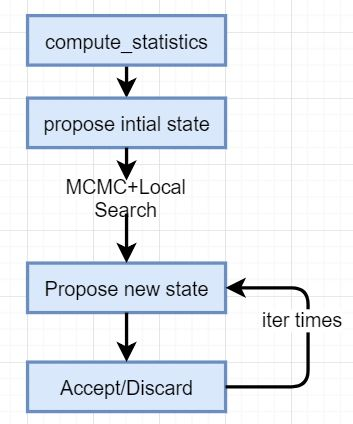
\includegraphics[width=7.5cm]{pic/process.jpg}}
\caption{The comparison of two methods with text length 3587(Left: original Right: variable exploring method)}
  \label{process}
\end{figure}
For time complexity, as shown in figure 3, we will analyse it step by step. Firstly, to have overall information for the text, it has the statistic analysis, and the time complexity is O(C+N). In the second step, it get a new state(a permutation) as the initial state, and it takes the time of O(N+C). Then there is our algorithm of MCMC and local search. It takes the iterations with number "iter", and in each iteration it get a new state which is also O(N+C). To determine whether accept the new state, it takes the time of O(C) and calculate the entropy. In conclusion, the time complexity is O(iter*(C+N)), and in fact as iteration number "iter" is a super-parameter, so in general it is in general in linear time complexity.
% \label{sec:proposed_model}
%
\section{Proposed Method}
MH algorithm is quite sophisticated. The formula, especially how to accept new permutation is unmodifiable, else the convergence would fail. Still, we come up with four ways to improve the performance of the algorithm, both on time and space. Some of them do work, which accelerate the convergence speed significantly. Also, some of them failed. They will all be introduced in the following part.
\subsection{Variable Exploring Method}
In the original version, each time the program walk one step by exchange two characters in current permutation. However, comparing to the whole state space(83!), exchanging two characters is a rather small step. You can think the state space in this way, an extremely large board. Each node on this board represents a permutation and it has a number on its head to tell you whether it is good or not--good permutations have a high score(In the program, a good one has a low entropy actually. But to explain the idea, we think it in this way, just for convenience). So, If you look down at the board of state space,you will find that most of the area is relatively flat with occasional small fluctuations and the area where correct solution lies is an imposing peak. Those permutations around the correct permutation also have a high score since they are only a little wrong. I draw a picture to illustrate this idea, which is showed in fig. 4. Then the exploring problem is kind of falling into finding this peak as quick as possible. However, when we start at a random place on this board, it may be a long distance from the beginning point to the peak. So we come up variable exploring method: we can stride at first, then we walk little step after we are close to the peak. 
\begin{figure}[htb]
\centerline{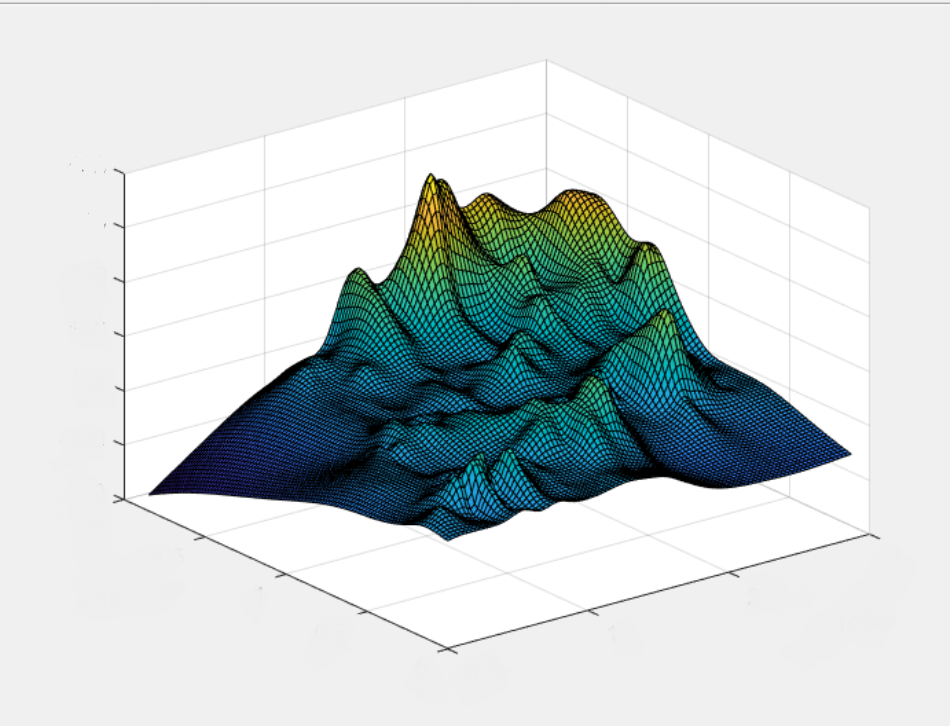
\includegraphics[width=7.5cm]{pic/solutionspace.png}}
\caption{How the state space look like, the top right corner is correct permutation which has high score.}
  \label{statespace}
\end{figure}

But here comes new question, how do we know we are at a good state or a bad state? After studying the nature of the state space, we find a property:
\newtheorem{myPro}{Property}

\begin{myPro}
    A good permutation is hard to stride while a bad permutation is easy to stride.
\end{myPro}
The reason is natural, if you are walking from a good state, which means you are walking to bad states. The larger the step is, the worse the new state is, meaning that that is hard to accept. The reason for walking from bad state is similar. Based on this property, we design our exploring algorithm in this way, showing as Algorithm 1
\begin{algorithm}[htb]
	\SetAlgoLined
	\KwResult{Sample set}
	initialization\;
	\While{not convergence}{
		step=3\;
		step\_count=15\;
		generate a new state according to step\;
		\eIf{accept}{
			//Renew step for new walk\\
			step=3\;
			record state\; 
			continue\;
		}
		{
			//Adjust walking step\\
			step\_count--\;
			step=step\_count/3\;	
		}
	}
	\caption{Variable exploring method}
\end{algorithm}
It's an adaptive algorithm, and the program automatically adjusts the number of steps as if it knows which kind of state it is. And this method works well!!!  The performance is showed in EXPERIMENT part.

\subsection{Memory Optimization}
Recording all the explored permutation seems to be a rather memory space consuming method. So we want to use local search only, which only record current permutation. However, this does not work at all. After 10000 times iterations, the text is still in chaos. So you can see the necessity of MH.

We analyze the reason why local search only fails. The algorithm is kind of soft, good state to bad state could be accepted sometimes. Although the correct permutation may be visited, it walked away soon. It's hard to stay at the correct state at the end of an iteration.

We also analyze the real memory space taken up. The iteration times in our version is 5000, so at most 5000 permutations will be recorded, just a constant number. We think that is acceptable.

\subsection{Double Search}
Before I introduce this problem, I want to start with three reasons why we're doing this.
\begin{itemize}
    \item In the original version, the state space is too large--83!. So we want to reduce it.
    \item In the transition probability matrix P, the items related to capital letters are small. This means that the rules may not be representative. Furthermore, in the final permutation, the decoding of capital letters may be inaccurate.
    \item Uppercase letters have certain connection with lowercase letters. This can be used to design heuristic function of transforming uppercase to lowercase.
\end{itemize}
So we come up with the idea double search. First, we find a match-up between  capital letters and lowercase letters. Then we are dealing with a smaller state space of 57!. The multiple of the reduction of the state space is considerable. Even in the worst case, that is, we go through all the uppercase-lowercase letters' match up. I show the calculation below. You can see the reduction factor $10^{21}$, that's a pretty big order of magnitude.
\begin{center}
    Original size of state space:$83!=3.946*10^{124}$\\
    New size of state space:$26!*57!=1.634*10^{103}$\\
    Reduction factor:$3.946^{124}/1.634^{103}=2.415*10^{21}$
    
\end{center}
Our new method reduces a big search problem to two small search problems. This also rises a problem, in the first step search, the program must find a correct match up, otherwise we will never find correct permutation in the second stage. This is still a challenge, and we're working on it.
\subsection{New Evaluation Function}
In order to make some improvements in the processes of getting to better states, we made some efforts to optimize the evaluation functions. Currently, we use the entropy of translated text according to the cipher key given by the current state, and decide whether accept the new state. We are motivated by the thought that the it may helps to optimize the exploring process and thus improve our overall performance.\\
We proposed a new evaluation function, which is to evaluate the "goodness", or "correctness" of our current translation. It is the probability that the consecutive letters make up correct words in the whole passage. However, we found that there are some problems in this evaluation: firstly we need a corpus containing the majority of words; secondly it may take long period of time to evaluate. Although the time complexity is still O(N), in practice it could cost a lot of time to refer to the corpus and try different possibilities of word matching. The evaluation method could be not so close to its real "correctness" because of the problems mentioned above. Even if these problems are properly addressed, there is another problem that we can predict that this evaluation is not smooth, or it scatters in a small range of values. Possibly there is a long time of low evaluation value before getting to the best state, and an abrupt increase near the best state. Thus. this evaluation function is not a good reference in our exploring, because it may mislead the exploring to take the states which are not so good  without realizing it. Thus, this effort was abandoned.\\
\label{sec:patterndeformations}

\section{Experiment}
\label{sec:results}
We have implemented the proposed models, used them to break the cipher and translate the cipher text of direct character substitution.  The results of our translated text 
are very convincing and run in real time. We have compared the translated text produced by our models and the original text.The results produced by our models are in qualitative agreement, not only in semantics, but also in the syntax, except for a few mistakes happening now and then.\\
\begin{table*}[ht]
    \centering
    \tabcolsep22pt
    \tbl{The experiments of our algorithm}{%
    \begin{tabular}{|c|c|c|c|c|}
    \hline  Type&Text Length&Entropy&Running$~$time(s)&Accuracy\\
    \hline  Narrative&489&1226.0018&22.29& 0.9627\\
    \hline Narrative&1982&4755.2851&39.09& 1.0\\
    \hline Narrative&8506&20418.7630&62.16&0.9976\\
    \hline Narrative&20011&50790.4921&84.13&0.9770\\
    \hline Narrative&52648&127245.5404&34.77&0.9949\\
    \hline Narrative&149906&360133.1816&139.16&0.9984\\
    \hline Narrative&324782&841088.7670&570.35&0.9974\\
    \hline Narrative(Uppercase)&850&2014.3251&30.92&0.9974\\
    \hline dialogue&3462&8789.4131&124.3363&0.9740\\
    \hline
    \end{tabular}}
\label{tab:symbols}
\begin{tabnote}
Several tries for different text type, text length and text form, and each experiments are given their entropy of their final result, the running time and the accuracy.
\end{tabnote}
\end{table*}
In our experiments, we set the text "war and peace" as the reference text. The test text we want to decipher is the paragraphs with different text length that are randomly chosen from the book "An Inquiry into the Nature and Causes of the Wealth of Nations", by Adam Smith.\\
In the result of our experiment, as shown in the table 1 below, we can find out that the accuracy of our result is relatively high(which are above 99\%) for text for different text length. There are several interesting findings during the process of our implementation, and some of which are not even expected before our implementation.\\
\begin{itemize}
    \item The result of our method depends on the reference text
    \item In the last but one experiment, we converted the whole text to the upper-case characters, and then run our algorithm to decipher our results. The result is unexpected: the semantics of the text is correct in general and the accuracy is very high(above 99\%), but the deciphered text is in the form of lower-case. We noticed that this is the case because the reference text is in the lower-case, and the therefore substitutions of characters are in lower case. We can speculate that if the reference text is all in upper case, then the result of deciphered text will be all in upper-case.
    \item We noticed that in the different types of texts, including narratives and dialogues, our methods performs equally well. In the last experiment, we used a piece of text from the book by Shakespeare, which is consist mainly of dialogues of characters. Although the reference text is in the form of narrative, our method still worked.\\
\end{itemize}
Besides, the method of variable exploring method that we proposed helped to speed up the process of convergence. We made another two experiments in the text length of 848 and 3587, respectively, and this trail we focus on the convergence process by watching its convergence graph. As shown in figure 5, with the text length 848, in the original version, it takes about 3000 steps to converge and get to a stable state, while in the process of our variable exploring method, it takes about 1500 steps, which are much more faster. Similarly, as shwon in figure 6 in the process of text length 3587, the original method suffers from the instability, with abrupt exploring, and long period of time without learning something useful, and the process of variable exploring method gives a more stable and continuous improving process.\\
\begin{itemize}
    \item 
\end{itemize}
\begin{figure}[htb]
\centerline{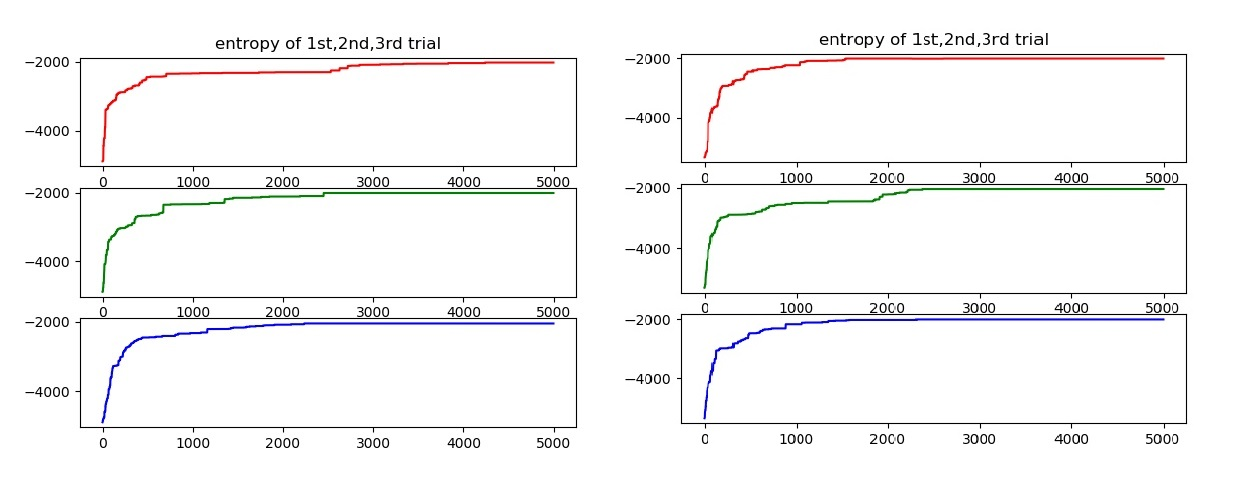
\includegraphics[width=9cm]{pic/compare848.jpg}}
\caption{The comparison of two methods with text length 848(Left: original Right: variable exploring method)}
\label{compare1}
\end{figure}

\begin{figure}[htb]
\centerline{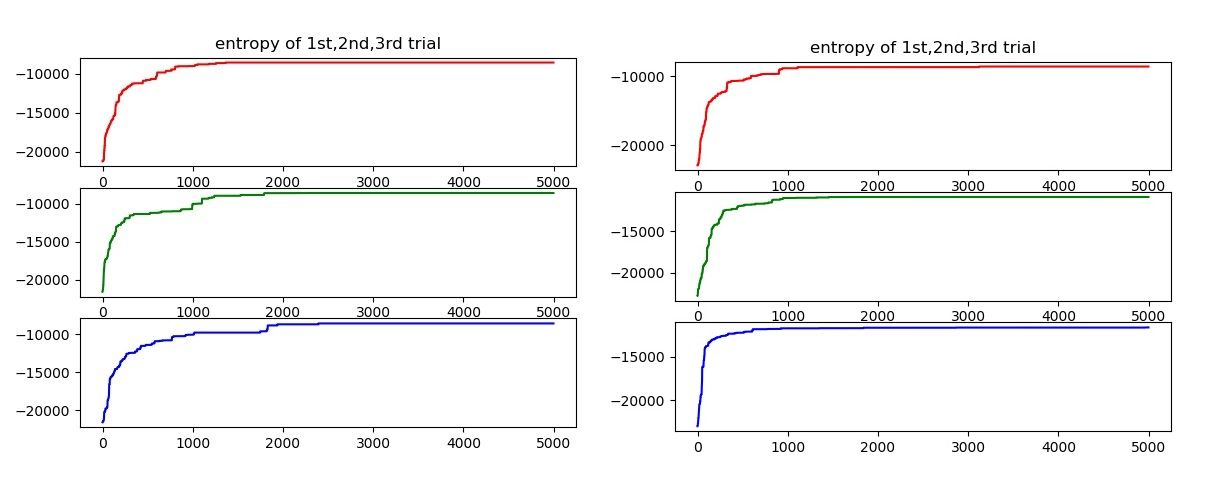
\includegraphics[width=9cm]{pic/compare3587.png}}
\caption{The comparison of two methods with text length 3587(Left: original Right: variable exploring method)}
  \label{compare2}
\end{figure}
However, we also noticed that there are some constraints in our algorithm:
\begin{itemize}
    \item As mentioned before, the performance of our algorithm depends on the quality of reference text. If the reference text is not in sufficient text length, or it does not contain enough statistical information of characters in words, the performance may be not as good as anticipated.
    \item We noticed that there is a problem in the text decipher: usually the first word in each paragraph starts with upper case characters, however, our algorithm sometimes cannot decode that upper-case character correctly. The reason is probably that there is not sufficient statistical information to tell our algorithm which can be a correct transformation between the upper-case to lower-case character. It is a possible solution to transform all the characters to the lower cases, but the syntax may be hurt a little bit.
    \item For the text with long enough text length, it takes a while to decode, and it may hurt the convenience of this decipher tool. In theory, our method is in linear time complexity, however, it takes much more steps to accept a new state, and it probably will not converge in the default step number(5000), and the result might not as good as anticipated. It is a choice to increase the number of max-steps when running this program, or just split the long text into several short text.
\end{itemize}
\section{Conclusion}
\label{sec:conclusion}
%
We have presented new models for text decryption of substitution cipher. Our method
combines and extends two-gram MCMC with local search methods, and had good performance on the accuracy and time complexity. The accuracy is above 99\% in our test set, and the time complexity is in linear with text length and alphabet length. Besides, we proposed new methods to address the current problems. The method of variable exploring method helps to find a better state, instead of the method of random walk, which speeds up the process of convergence significantly. The method of double search divides the searching process into two parts, therefore reduce the search space exponentially. We also made some efforts to optimize and save the memory usage, and try new evaluation functions to better find out where we are in the process to have a good translation. 
% \appendix

% \section{Classical Multidimensional Scaling}





% Bibliography
% \bibliographystyle{plain}
% \bibliography{}
\begin{thebibliography}{1}
\bibitem{Conner} Conner, S. (2003). Simulation and solving substitution codes. Master's thesis, Department of Statistics, University of Warwick.
\bibitem{Ravi} Ravi, S., \& Knight, K. (2008, October). Attacking decipherment problems optimally with low-order n-gram models. In proceedings of the conference on Empirical Methods in Natural Language Processing (pp. 812-819). Association for Computational Linguistics.
\bibitem{Nuhn} Nuhn, M., Schamper, J., \& Ney, H. (2013). Beam search for solving substitution ciphers. In Proceedings of the 51st Annual Meeting of the Association for Computational Linguistics (Volume 1: Long Papers) (Vol. 1, pp. 1568-1576).
\bibitem{Hauer} Hauer, B., Hayward, R., \& Kondrak, G. (2014). Solving substitution ciphers with combined language models. In Proceedings of COLING 2014, the 25th International Conference on Computational Linguistics: Technical Papers (pp. 2314-2325).
\end{thebibliography}
                                % Sample .bib file with references that match those in
                                % the 'Specifications Document (V1.5)' as well containing
                                % 'legacy' bibs and bibs with 'alternate codings'.
                                % Gerry Murray - March 2012

% \received{September 2008}{March 2009}

\end{document}
% End of v2-acmtog-sample.tex (March 2012) - Gerry Murray, ACM
